\chapter{Software}
\label{chapter3}

\section{Support de la caméra}

Pour gérer les différentes configurations matérielles de façon plus "userfriendly", la Raspberry Pi dispose d'un fichier de configuration \codeinline{text}{config.txt} que le $bootloader$ interprétera pour sélectionner les $overlays$ correspondants et composer le $devicetree$ qui convient à l'architecture matérielle utilisée. Celui-ci étant ensuite passé au $kernel$ lors du démarrage.

%\vspace{1cm}

Cette subtilité propre aux Raspberry Pi permet à l'utilisateur de ne pas avoir besoin d'avoir affaire au $devicetree$ quand il s'agit de configuration. Par exemple l'activation du support d'un élément courant sur les Raspberry Pi comme le module Raspicam.

%\vspace{1cm}

le logiciel \codeinline{text}{raspi-config} n'est autre qu'une interface à ce fichier de configuration.

\vspace{1cm}

Pour activer le support matériel de la caméra, il faut ajouter les lignes suivantes à ce fichier~:

%\code{ruby}
\code{bash}
start_x=1
gpu_mem=128
\end{minted}

À travers Yocto, cela passe par l'ajout des lignes ci-dessous au fichier \codeinline{text}{local.conf} et donc à son modèle le fichier \codeinline{text}{meta-autoscope/conf/local.conf.sample} dans la $layer$ dédiée au projet.

\code{ruby}
VIDEO_CAMERA = "1"
GPU_MEM = "128"
\end{minted}

\vspace{1cm}

Quant à l'utilisation de la caméra, il existe des logiciels tels que \codeinline{text}{raspivid} pour filmer ou \codeinline{text}{raspistill} pour prendre des clichés. Tous deux font partie de la suite \codeinline{text}{userland} que l'on ajoute à notre image via la ligne ci-dessous dans le fichier\\\codeinline{text}{meta-autoscope/recipes-autoscope/images/autoscope-console-image.bb}~:

\code{ruby}
IMAGE_INSTALL += "userland"
\end{minted}

À l'usage, la commande suivante permet d'afficher en plein écran le flux vidéo jusqu'à ce qu'on le stoppe~:

\code{bash}
~$ raspivid -t 0
\end{minted}

\section{Étude de l'embarcation de Stellarium}

Une première évaluation de la faisabilité de l'embarcation de Stellarium sur la Raspberry Pi a été de l'installer via le gestionnaire de paquet sur une Raspberry Pi dotée de Raspbian.

\code{bash}
~$ sudo apt-get install stellarium
\end{minted}

\vspace{1cm}

Avec le compositeur graphique logiciel, Stellarium est totalement inutilisable. Cependant il est possible d'activer le compositeur graphique matériel. Pour cela il faut activer l'option \codeinline{text}{Advanced Options -> GL Driver} dans le menu \codeinline{text}{raspi-config}.

La différence de rendu peut être observée avec l'outil \codeinline{text}{glxgears} prévu à cet effet. Celui-ci s'installe par la ligne suivante~:

\code{bash}
~$ sudo apt-get install mesa-utils
\end{minted}

\begin{figure}[H]
    \centering
    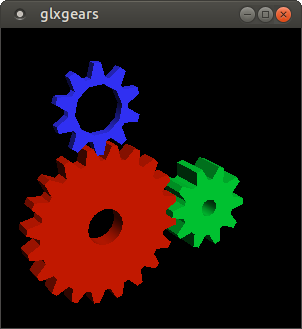
\includegraphics[width=0.3\linewidth]{\figures/photo_glxgears.png}
    \decoRule
    \caption[
    Captures d'écran de glxgears]{
    Captures d'écran de glxgears}
    \label{fig:Captures d'écran de glxgears}
    \end{figure}

\vspace{1cm}

Le résultat est alors meilleur, Stellarium est utilisable bien qu'il lui arrive de planter lorsque l'on fait un déplacement trop brusque dans le ciel.

\vspace{1cm}

Il existe une version mobile de Stellarium disponible notament pour Android et iOS qui est une version allélégée et optimisée pour l'usage sur un smartphone.

Ses sources sont disponibles à l'adresse suivante~:\\\url{https://noctua-software.com/stellarium-mobile}

\vspace{1cm}

Il semble que cette version puisse fonctionner telle quelle sur Linux. À l'heure actuelle nous n'avons pas réussi à compiler Stellarium mobile pour un problème de dépendance à une librairie (Qt5Declarative, faisant partie du paquet qtdeclarative5-dev) qui n'existe plus dans les versions récentes de Qt, ultérieures à la version Qt5.6 pour être précis.

Le problème pourrait sans doute être résolu en récupérant ladite librairie dans les dépots d'une distribution plus ancienne, Ubuntu Xenial (Qt5.5.1) ou Trusty (Qt5.2.1) par exemple.

